\documentclass[14pt]{article}
\usepackage{amsmath,amsthm,amsfonts,amssymb,tikz,scalerel,mathrsfs,marvosym,titlesec,leftidx}

\usepackage{tikz}
\def\layersep{2.5cm}
\usepackage[all]{xy}
\usepackage{fancyhdr}
\usepackage{blkarray}
\usepackage{adjustbox}
\usepackage{hyperref}
\usepackage[linesnumbered,ruled]{algorithm2e}
\usetikzlibrary{arrows.meta}
\usepackage[font=small,labelfont=bf,tableposition=top]{caption}



\DeclareCaptionLabelFormat{andtable}{#1~#2  \&  \tablename~\thetable}

\theoremstyle{plain}
\newtheorem{corollary}{Corollary}[subsection]
\newtheorem{convention}[corollary]{Convention}
\newtheorem{example}[corollary]{Example}
\newtheorem*{theorem*}{theorem}
\newtheorem{theorem}[corollary]{Theorem}
\newtheorem{lemma}[corollary]{Lemma}
\newtheorem*{lemma*}{Lemma}
\newtheorem{maintheorem}{Theorem}
%reset maintheorem counter to use the corresponding letter
\renewcommand{\themaintheorem}{\Alph{maintheorem}}
\newtheorem{remark}[corollary]{Remark}
\newtheorem{proposition}[corollary]{Proposition}


\theoremstyle{definition}
\newtheorem{definition}[corollary]{Definition}
\newtheorem{definition*}{Definition}

%change the default font to bodoni
\usepackage[default]{gfsbodoni}
\usepackage[T1]{fontenc}



%start at section 0 for introduction 
\setcounter{section}{-1}
\newcommand{\un}{\textunderscore}
\newcommand{\A}{\mathcal{A}}
\newcommand{\abs}[1]{\vert #1 \vert }
\DeclareMathOperator{\ad}{ad}
\DeclareMathOperator{\Aut}{Aut}
\renewcommand{\b}{\bullet}
\newcommand{\bp}{\mathbf{\Pi}}
\newcommand{\bl}[2]{\left\langle #1,#2\right\rangle}
\def\BVm{\operatorname{BV}_-}
\DeclareMathOperator{\BiMod}{BiMod}
\DeclareMathOperator{\bimod}{bimod}
\newcommand{\C}{{\mathcal{C}}}
\DeclareMathOperator{\CC}{CC}
\def\cd{\operatorname {cd}}
\DeclareMathOperator{\ch}{ch}
\DeclareMathOperator{\CH}{CH}
\DeclareMathOperator{\coh}{coh}
\DeclareMathOperator{\cone}{cone}
\DeclareMathOperator{\coker}{coker}
\renewcommand{\d}[1]{\mathbb{#1}}
\newcommand{\D}{{\mathscr{D}}}
\DeclareMathOperator{\der}{R}
\DeclareMathOperator{\Def}{Def}
\newcommand{\define}{\stackrel{\operatorname{def}}{=}}
\let\div\relax %unassign \div
\DeclareMathOperator{\div}{div}
\DeclareMathOperator{\divu}{div}
\newcommand{\ds}{\oplus}
\newcommand{\DS}{\bigoplus}
\newcommand{\epi}{\xymatrix{{}\ar@{->>}[r]&{}}}
\DeclareMathOperator{\End}{End}
\DeclareMathOperator{\Ext}{Ext}
\newcommand{\f}[1]{\mathfrak{#1}}
\DeclareMathOperator{\fd}{fd}
\newcommand{\fC}{\f{C}}
\newcommand{\fD}{\f{D}}
\newcommand{\floor}[1]{\left\lfloor #1 \right\rfloor}
\newcommand{\fun}{\mapsto}
\newcommand{\dgg}{{\f{g}^\bullet}}
\newcommand{\g}{\f{g}}
\DeclareMathOperator{\Gd}{Gd}
\DeclareMathOperator{\Gr}{Gr}
\DeclareMathOperator{\gldim}{gl.dim}
\let\H\relax %unassign \H
\DeclareMathOperator{\H}{H}
\DeclareMathOperator{\HH}{HH}
\DeclareMathOperator{\HC}{HC}
\DeclareMathOperator{\Hom}{Hom}
\DeclareMathOperator{\Id}{Id}
\DeclareMathOperator{\im}{im}
\newcommand{\iso}{\stackrel{\sim}{\longrightarrow}}
\DeclareMathOperator{\Jac}{Jac}
\renewcommand{\k}{\Bbbk}
\newcommand{\K}{\mathbb{K}}
\DeclareMathOperator{\length}{length}
\DeclareMathOperator{\lrk}{\l.rk}
\newcommand{\leftperp}[1]{\leftidx{^\perp}{#1}}
\newcommand{\m}{\f{m}}
\DeclareMathOperator{\MCM}{MCM}
\DeclareMathOperator{\MC}{MC}
\DeclareMathOperator{\MCcal}{\mathcal{MC}}
\DeclareMathOperator{\Mod}{Mod}
\DeclareMathOperator{\Mor}{Mor}
\def\mod{\operatorname{mod}}
\newcommand{\mor}{\longrightarrow}
\DeclareMathOperator{\Test}{Test}
\newcommand{\T}{\mathscr{T}}
\renewcommand{\O}{\mathcal{O}}
\DeclareMathOperator{\NS}{NS}
\DeclareMathOperator{\Num}{Num}
\newcommand{\p}{\mathfrak{p}}
\DeclareMathOperator{\per}{per}
\DeclareMathOperator{\Ob}{Ob}
\DeclareMathOperator{\Perf}{Perf}
\DeclareMathOperator{\Pic}{Pic}
\DeclareMathOperator{\Proj}{Proj}
\DeclareMathOperator{\poly}{poly}
\DeclareMathOperator{\Qcoh}{Qcoh}
\DeclareMathOperator{\QGr}{QGr}
\DeclareMathOperator{\RHom}{RHom}
\renewcommand{\r}[1]{\mathcal{#1}}
\DeclareMathOperator{\rk}{rk}
\DeclareMathOperator{\rrk}{r.rk}
\def\locExt{\mathscr{E}\mathit{xt}}
\DeclareMathOperator{\SL}{SL}
\DeclareMathOperator{\SPS}{SPS}
\DeclareMathOperator{\sing}{sing}
\DeclareMathOperator{\vectorspan}{span}
\DeclareMathOperator{\Spec}{Spec}
\DeclareMathOperator{\Supp}{Supp}
\DeclareMathOperator{\SupVec}{SupVec}
\DeclareMathOperator{\Sym}{Sym}
\def\locHom{\operatorname {\mathscr{H}\mathit{om}}}
\DeclareMathOperator{\Tails}{Tails}
\def\ltr{\overset{L}{\tr}}
\renewcommand{\r}[1]{\mathcal{#1}}
\newcommand{\mono}{\xymatrix{{}\ar@{^{(}->}[r]&{}}}\DeclareMathOperator{\num}{num}
\DeclareMathOperator{\rad}{rad}
\DeclareMathOperator{\Tor}{Tor}
\DeclareMathOperator{\Tors}{Tors}
\newcommand{\tr}{\otimes}
\newcommand{\trps}[1]{ \leftidx{^{\operatorname{tr}}}{#1}}
\def\uRHom{\operatorname {R\mathcal{H}\mathit{om}}}
\newcommand{\w}{{\tt{w}}}
\newcommand{\Q}{\mathbb{Q}}
\DeclareMathOperator{\qis}{qis}
\DeclareMathOperator{\Qvr}{\mathcal{Q}}
\newcommand{\Z}{\mathbb{Z}}


%add dots between section and page in toc
\usepackage{tocloft}
\renewcommand{\cftsecleader}{\cftdotfill{\cftdotsep}}


%interline a little larger
\linespread{1.28}

%change the dimensions of the margin
\usepackage{geometry}
 \geometry{
 a4paper,
 total={210mm,297mm},
 left=23mm,
 right=23mm,
 top=32mm,
 bottom=20mm,
 }
 
%changeqedsymbol
\renewcommand{\qedsymbol}{\CrossedBox}

%make the (sub)subsections run into the text, the 0.25 is the distance between the numbering and title
\titleformat{\subsubsection}[runin]{\normalfont\normalsize\bfseries}{\thesubsubsection.}{0.25em}{}
\begin{document}
\title{\textbf{DETECTING FORGED BANKNOTES}}
\author{LOUIS DE THANHOFFER DE VOLCSEY}
\date{\emph{september 2017}}
\maketitle	
\vspace{1in}
%add header on other pages

\pagestyle{fancy}
 \rhead{LdTdV}
\chead{{\large{\bf Detecting forged banknotes}}} \lfoot{} \rfoot{\bf  page \thepage} \cfoot{}

\noindent\hrulefill
\tableofcontents{}
\noindent\hrulefill
\newpage 
\section{Introduction}
\subsection{Overview}
In this project we design a neural net capable of reliably detecting forged banknotes.\\ Our algorithm relies on data that was collected by scanning notes which were then processed statistically. In doing this, one is able to distill some of the key features that describe the inherent mathematical information inherent to each image.\\ 
Our approach can be subdivided in two major phases:
\begin{enumerate}
\item {\bf reengineering the data}. Based on the famous machine learning folklore:
\begin{center}
\emph{machine learning starts with feature engineering,}	
\end{center}
we perform an extensive analysis of the data through various statistical tools before fitting it to a neural net. 
Some of the techniques we use include:  detecting and removing outliers, describing the various relations between different features, visualizing the data in  3d and 2d  as well as analyzing to what extend the data can be separated by a decision boundary.\footnote{we refer the reader to \S ref{conc1} for a more technical overview account of these techniques }
\item
{\bf Designing a neural network}
Once the data has been analyzed, we use the \texttt{keras} Python library to implement a neural net. To this end, we initially consider a rather simple model and analyze its performance through the use of learning curves. These curves give us not only an insight into how well the neural net can handle the problem, but they allow us to understand how to make modifications in order to improve on the design. Our final model will be capable of  accurately detecting forged banknotes {\bf 99\%} of the time all the while retaining a simple and transparent architecture.
\end{enumerate}
\subsection{Background to the problem}
Known  colloquially as one of the \emph{worlds second oldest profession} \cite{wikiprof}, the art of counterfeiting legal tender dates back to the invention of money itself. From forgers reproducing gold coins in Roman times by using cheaper base metals \cite{wikiforge} to the use of Mulberry trees \cite{wikiforge} in order to imitate banknotes in 13th century China, forgers and governments have always played a fiendish cat-and-mouse game that makes for a fascinating history. Counterfeiting techniques were even used as a form of warfare in the U.S. Revolutionary war by the British in order to devaluate the newly created U.S. dollar \cite{wikiforge}.\\
The problem of counterfeiting however, is not just one of historical importance. In fact, it is estimated that this issue produces an annual increase in inflation that results in a loss of purchasing power of over 250 billion dollar annually to the U.S. economy \cite{usforge}.\\ 
In modern times, the techniques to detect forgery have grown very subtle as anti-counterfeiting measures enter the 21st century (see \cite{wikiforge}), ranging from the use of complicated printing techniques to the inclusion of watermarks. The main paradigm behind these techniques has however remained unchanged throughout history:  at its core, a note is fitted with a set of attributes and run through a series of tests to determine if those attributes are indeed present .\\This project aims to use state-of-the art machine learning techniques to detect forgery in an entirely different way. Instead, using mathematical analysis, the banknote will inherently be described in waveform. We will subsequently use the technology of neural nets to devise a formula which uses some inherent statistical features of this wave allowing us to detect forgery.

\section{Analyzing the dataset}
The dataset in question was extracted from the UC Irvine machine learning repository \footnote{\url{https://archive.ics.uci.edu/ml/datasets/banknote+authentication}}. It serves as the basis for a regression analysis performed by Gillich and Lowesh in \cite{BNA}. In loc. sit. the authors scanned a set of 1372 banknotes into 400$\times$ 400 pixels  and applied a \emph{Wavelet transform} to each image. The wavelet transform is a mathematical tools which finds its origins in the theory of Fourier transforms and allows one to encode image data very efficiently. For our purposes it will be sufficient to know that it compresses an image by extracting coefficients according to an underlying probability distribution. The features of the dataset in question consist of a description of 4 statistical properties of this distribution:
\begin{enumerate}
\item the variance
\item the skewness
\item the kurtosis	
\item the Shannon entropy
\end{enumerate}
Additionaly, to each feature a binary label is associated indicating whether or notethe note is real or counterfeit (0=real, 1=fake). In the dataset, the first 762 notes are real, whereas the last 610 are counterfeit. By way of example, the 350'th datapoint is the $5$-tuple:

\begin{center}
\texttt{[-1.5768,10.843,2.5462,-2.9362,0]
}	
\end{center}
\subsection{a First exploration}
We begin by describing the basic statistical properties of the data. These are listed below as well as displayed graphically in the form of a boxplot:
\begin{table}[ht]
\begin{minipage}[b]{0.56\linewidth}
\centering
\begin{tabular}{|c| c| c |c |c|}
\hline
\texttt{statistic} & \texttt{variance} &\texttt{skewness}&\texttt{curtosis}  &\texttt{entropy} \\
	\hline
         mean &    0.43 &   1.92 &   1.40  & -1.19\\
         \hline
         std  &    2.84  &   5.87  &   4.31   &  2.10\\
         \hline
         min  &    -7.042 & -13.77  & -5.29    & -8.55\\
         \hline
         25\% &   -1.77  &  -1.71  &   -1.57  & -2.41\\
         \hline
         50\% &   0.50 &  2.32   &  0.62    &  -0.59\\
         \hline
         75\% &   2.82   &  6.81   &  3.18    &  0.39\\
         \hline
         max  &    6.82  &  12.95  &  17.93   &  2.45\\
         \hline
 \end{tabular}   
 \caption{describing the data}
    \label{table:student}
\end{minipage}\hfill
\begin{minipage}[b]{0.4\linewidth}
\centering
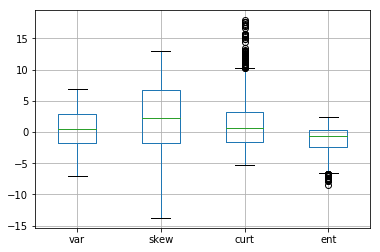
\includegraphics[width=67mm]{banknote_forgery_files/banknote_forgery_9_0}
\captionof{figure}{the boxplot of the data}
\label{boxplot}
\end{minipage}
\end{table}

\noindent We see that all $4$ features have rather similar statistical properties. As a result we opt to not renormalize the data, preferring to keep transparency\\ 
A closer look at the boxplot does yield an interesting observation: it seems that a significant number of datapoints have a kurtosis lying above the boxplot whiskers. These should be considered outliers. Similarly, the entropy feature, seems to present a significant number of outliersas well.\\ After counting these, we removed a total of {\bf 65} datapoints (equivalent to {\bf 4.3\%} of the total data).\\ 
The new dataset now consist of {\bf 1305} entries and presents no outliers.
\subsection{the Correlation between features} The next step in our data exploration, consists of investigating the possible correlations between mutual features. This is an important step as correlated features morally correspond to redundant information, which may cause overfitting as we build a model later on.\\ The Pearson correlation coefficients for each choice of feature pair together with their respective scatterplots  are listed below. \footnote{we note that in the case where two identical features are chosen, their histogram is displayed}
\begin{table}[ht]
\begin{minipage}[b]{0.4\linewidth}
\centering
\begin{tabular}{|c |c| c| c |c |}
\hline
feature  &         var   &   skew &     curt    &   ent\\
  \hline
var &   1 & 0.26 & -0.38 & 0.27\\
\hline
skew & 0.26 & 1 & -0.78 & -0.52\\
\hline
curt & -0.38 & -0.78 &  1  & 0.32\\
\hline
ent   & 0.27 & -0.52 &  0.32 &  1\\
\hline
\end{tabular}
\vspace{0.83in}
 \caption{the Pearson correlation matrix}
    \label{table:student}
\end{minipage}
\begin{minipage}[b]{0.445\linewidth}
\centering
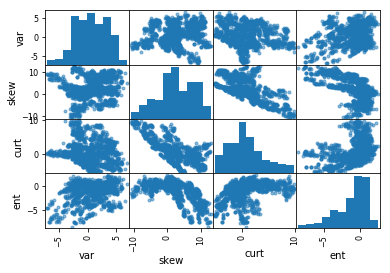
\includegraphics[width=95mm]{banknote_forgery_files/banknote_forgery_15_1}
\captionof{figure}{the scatterplot of the features}
\label{boxplot}
\end{minipage}
\end{table}

 \noindent Both the Pearson matrix and the scatterplot indicate that exactly two features are significantly correlated: kurtosis and skewness.\\ Comparing these features, yields a Pearson correlation of 78\% in absolute value. Additionally, the scatterplot shows that linear trend seems to form around the $y=-x$ axis between those features.\\ 
 We choose however to keep those features as removing either would come  at the cost of significantly reducing the dataspace,  which in turn could impact the predictive capabilities of the final model. Instead, since we intend to analyze the model through learning curves later on we will be able to detect overfitting as a difference in behavior between training and testing accuracy and will adapt the model accordingly if necessary. 

\subsection{Reducing the dimension} The third step in our analysis consists of reducing the dimension of the features to $3d$ and $2d$. The tool of choice for such problems is a \emph{principal component analysis}, This method determines an optimal subspace by maximizing variance (or equivalently minimizing mean squared error), subsequently exhibits an orthonormal basis for this subspace. From there, the coordinates for any projected vector with respect to this basis are computed and returned. For the reader's benefit. A pseudo-algorithm of this procedure in sklearn is given below: 
\begin{algorithm}\label{PCAalg}
    \SetKwInOut{Input}{Input}
    \SetKwInOut{Output}{Output}

    \underline{function reduce} $(\textrm{features}, d)$\;
    \Input{a set of features together with the desired final dimension}
    \Output{a set of $d$-dimensional features, together with the total variance of each dimension}
    pca=PCA(n\textunderscore features=$d$) \\
  	pca.fit(features)\\
    print(pca.explained\textunderscore variance\textunderscore ratio\textunderscore)	\\
   reduced\textunderscore data=pca.transform(features)\\
   return reduced\un data      
   \caption{reduce dimensionality using PCA }
\end{algorithm}

\noindent The total variance for each principal component after applying a PCA transformation is listed below:\\
\begin{center}
\begin{tabular}{|c|c|c|c|c|}
	\hline
	component & 1 & 2 & 3& 4\\
	\hline
	expl. var.& 76\%&  14\% & 6\% & 3\%\\
	 \hline
\end{tabular}
\end{center}
    
   
    
\subsection{Plotting the data}\label{SVM1} Reducing the dimensions of the features allows us to observe how the binary labels are distributed. In the figures below, the features were reduced using the \underline{reduce} function and then plotted. The red labels correspond to real banknotes whereas the green labels represent forgeries.

\begin{table}[ht]
\begin{minipage}[b]{0.56\linewidth}
\centering
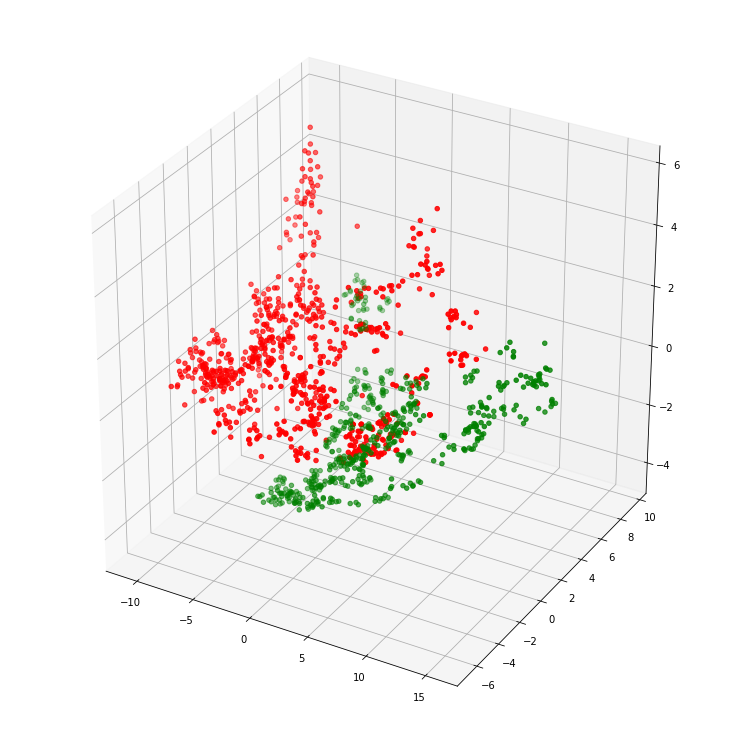
\includegraphics[width=90mm]{banknote_forgery_files/model_1}
 \caption{the 3d reduced data}
    \label{table:student}
\end{minipage}\hfill
\begin{minipage}[b]{0.4\linewidth}
\centering
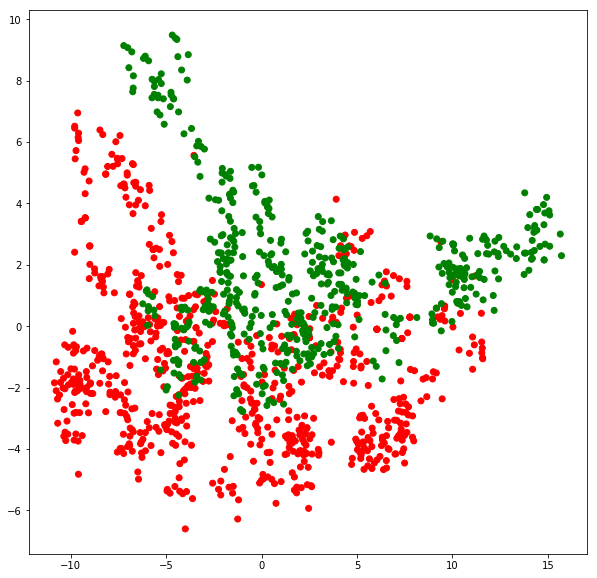
\includegraphics[width=70mm]{banknote_forgery_files/model_2}
\vspace{0.29in}
\captionof{figure}{the 2d reduced data}
\label{boxplot}
\end{minipage}
\end{table}

\noindent These plots indicate that the reduced data is not linearly separable. What's more, a conclusive decision boundary is difficult to discern. This hypothesis can be confirmed numerically through the use of a support vector machine. This clustering tool maximizes the \emph{marginal distance} between two classes of datapoints  in order to compute a hyperplane which separates them optimally. In particular, should the classes be linearly separable, the accuracy of the algorithm would be 100\%.\\ 
Below, we first apply the \underline{reduce} function described in {\bf Algorithm 1} and then fit a support vector machine and compute its accuracy -which in this case simply the relative number of correctly classified points:
     \begin{algorithm}
    \SetKwInOut{Input}{Input}
    \SetKwInOut{Output}{Output}

    \underline{function lin \un sep\un acc} $(\textrm{features},m)$\;
    \Input{a set of features}
    \Output{the accuracy of a separating hyperplane after reducing dimensions up to $m$}
    d=features.shape[1]\\
    \For{i in range(\textrm{m,d+1}) }{reduced\un features=reduce(features,$i$)\\

    	clf=SVC$()$\\
		clf.fit(reduced\un features,labels)\\
		predicted\un labels=clf.predict(reduced\un features)\\
		accuracy\un score(predicted\un labels,labels)\\
		}      
   \caption{compute the accuracy of a separating hyperplane after reducing dimensions}
\end{algorithm}

The results of this algorithm are listed in the table below:
\begin{center}
\begin{tabular}{|c|c|c|c|}
	\hline
	dimension & 4 & 3 & 2\\ 
	\hline 
	accuracy & 81\% & 78\% & 59\%\\
	\hline
\end{tabular}
\end{center}
  This indeed confirms our hypothesis that the data cannot be linearly separated, even after reducing dimensions.\\ It is worth noting that one could alternatively implement a support vector machine with a more sophisticated kernel that separates the data using more general algebraic varieties for instance. It turns out that -for example- allowing for a cubic kernel does not improve the accuracy as the table below shows:
\begin{center}
\begin{tabular}{|c|c|c|c|}
	\hline
	dimension & 4 & 3 & 2\\ 
	\hline 
	accuracy & 81\% & 78\% & 42\%\\
	\hline
\end{tabular}
\end{center}


 \subsection{Conclusions}\label{conc1}
Our analysis of the data has let us to the following conclusions:
\begin{itemize}
\item The dataset -consisting of $4$ features with binary labels-  is roughly equidistributed. As such it is not necessary to perform any rescaling operation.
\item A closer look at the boxplot does show outliers however. After removing these, 95.7\% of the mass is retained.
\item Within the data, two features are heavily correlated: computing the Pearson coefficient of kurtosis vs. skewness results in a $\vert 72\%\vert $ correlation. This could be a possible explanation of overfitting later on.
\item Applying a principal component analysis allows us to reduce the data to 3 or 2 dimensions and to conclude that the distribution of the labels is rather heterogeneous. In particular the data does not present an obvious decision boundary.
\item Fitting a support vector machine (possibly after reducing dimensions) supports this evidence as this results in misclassification about 20\% of the time.
\end{itemize}

\section{Building a neural net}
The analysis in the previous section led us to the conclusion that the dataset is potentially vulnerable to overfitting and that a simple decision boundary does not exist. In light of these facts, we opt to use a neural network to classify the data, as these are known to be both robust enough to handle more complicated datasets and transparent enough in their design.
\subsection{Neural nets in Keras} 

To implement a neural net, we will  use the \texttt{keras} Python library using a \texttt{TensorFlow} backend. This library (built specifically for neural nets) has become one of the gold standards in the industry due to its ease of use and its modularity. In fact, the programming paradigm in \texttt{keras} is remarkably streamlined: in short, a network is built in two steps:
\begin{itemize}
\item {\bf step 1} the user designs the net layer by layer. For each layer they can easily specify a chosen number of input nodes, an activation function or implement regularization functionalities such as dropout.
\item{\bf step 2} The design is subsequently compiled and fitted to a given training/testing set using a gradient descent method. One pleasant feature of \texttt{keras} is that the parameters of the gradient descent method can easily be tweaked, which results in a highly customizable optimizer.
\end{itemize}
As was mentioned in the introduction, our approach will be to start with a rather coarse neural net and refine the design as we make conclusions based off the resulting learning curves. To streamline the code, we chose to implement {\bf step 2} as a separate function. To this end we first split the data into a training $(2/3)$ and testing $(1/3)$ set.\footnote{ As a technical note, we warn the reader that numpy data needs to be transformed slightly in order to make it compatible with keras: the features need to be converted into matrices and the labels need to be one-hot-encoded}.\\ The algorithm below fits a neural net using this training/testing set according to a prescribed model with a specified number of epochs and choice of optimizer: 
\begin{algorithm}

    \SetKwInOut{Input}{Input}
    \SetKwInOut{Output}{Output}

    \underline{comp\un fit}(model, epochs, sgd)\;
    \Input{a \texttt{keras} neural net, a number of epochs, a gradient descent optimizer}
    \Output{a fitted model}
model.compile( optimizer=sgd, loss='categorical\un crossentropy', metrics=['accuracy'])\\
fm=model.fit(x\un train, y\un train, validation\un data=(x\un test, y\un test), epochs=epochs,batch\un size=10)\\
return fm
   \caption{compile and fit a neural net }
\end{algorithm}

\noindent As part of our preparatory work, a function \underline{learning\un curves} was implemented as well. This function displays both the accuracy and the value of the loss function for training and testing sets after each individual epoch.

\subsection{Finding the right model}

\subsubsection{A coarse model}\label{coarse}
We begin our search for the optimal model with a standard implementation of logistic regression. This neural net has no hidden layers and uses a sigmoid activation function. For the benefit of the reader we describe an implementation of this neural net using the standard \texttt{rmsprop} optimizer with 300 epochs:
\begin{algorithm}
    \SetKwInOut{Output}{Output}
	log\un model$()$\;
    \Output{a a fitted  model for logistic regression together with the learning curves}
    log\un model=Sequential$()$\\
	log\un model.add(Dense(2,input\un dim=4,activation='sigmoid'))\\
	history=comp\un fit(logmodel,'rmsprop',300)\\
	learning\un curves(history)\\
   \caption{logistic regression in \texttt{keras} }
\end{algorithm}

The learning curves for this model are displayed below
\begin{table}[ht]
\begin{minipage}[b]{0.3\linewidth}
\centering
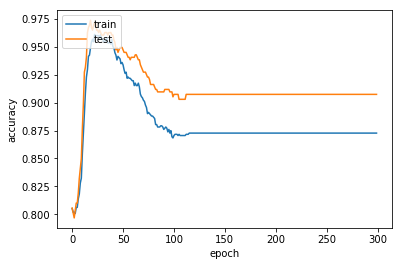
\includegraphics[width=80mm]{banknote_forgery_files/logmodel_1}
\end{minipage}\hfill
\begin{minipage}[b]{0.5\linewidth}
\centering
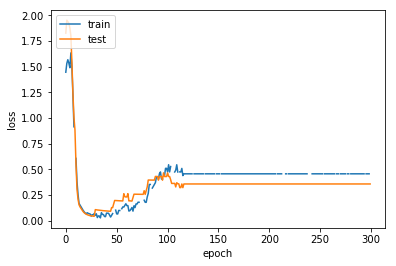
\includegraphics[width=80mm]{banknote_forgery_files/logmodel_2}
\end{minipage}
\end{table}

Through these learning curves, we are able to draw a number of conclusions:
\begin{enumerate}
\item the final accuracy on the training set is 86\% . This does not improve significantly on the 81\% accuracy of the support vector machine discussed in \S 1.\ref{SVM1}, or in other words, the model is underfitted as well. This points to the fact that our coarse model is too basic to handle the dataset. To remedy this, we will investigate how the results change as we add hidden layers to the net in \S2.\ref{final} .
\item The learning accuracy on the testing set is 90\&, implying that the algorithm will still misclassify one out ten new banknotes.\footnote{we note that a comparison with the SVM cannot be made here as it was not tested on new examples. Instead we took the complete dataset into account to conclude that the data could not be separated linearly}  
\item We also see a nonnegligable difference between both training and testing accuracies. In particular, the testing set has a higher accuracy than the training set, which doesn't typically happen. Since our dataset is comparatively small, this could be a result of how the the data was split. To account for this, we altered the seed for the pseudorandom generator used to split the data.
\item Both in the case of training and testing, the loss stagnates at around 0.4/0.5 after 110 epochs. As a result, the accuracy stagnates as well since the algorithm is no longer optimizing itself. Geometrically speaking, the optimizer has stumbled upon a value that is a local minimum for the cost function. This value is arguably still rather high as the function has only dropped around 80\%. As part of our exploration,  we will tweak the parameters of the optimizer to see if this result in a more efficient gradient descent method in the paragraph below:
\end{enumerate}

\subsubsection{Optimizing the optimizer}
Tweaking the parameters of the optimizer in the previous model can be done mutatis mutandis by replacing the default \texttt{rmsprop}  in line 4 of {\bf algorithm 4} by a custom one using the command \texttt{SGD.optimizers()} and specifying the chosen parameters. The analysis done in \S 2.\ref{coarse} points to the fact that -for example- decreasing the learning rate could improve the accuracy as it would give the optimizer more freedom to "explore" before it finds a local minimum. After a few trials with different learning rates, we found that the \texttt{Adam} optimizer built into \texttt{keras} -whose learning rate is one tenth of \texttt{rmsprop} indeed showed some improvment. The learning curves for this model are displayed below:  
 \begin{table}[ht]
\begin{minipage}[b]{0.3\linewidth}
\centering
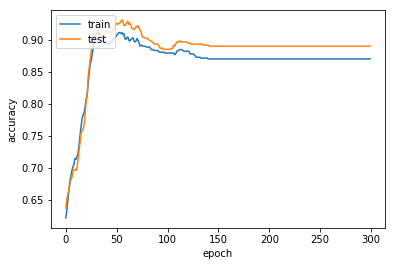
\includegraphics[width=80mm]{banknote_forgery_files/adam_model_1}
\end{minipage}\hfill
\begin{minipage}[b]{0.5\linewidth}
\centering
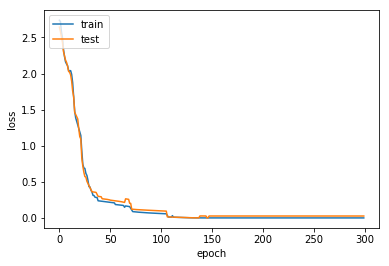
\includegraphics[width=80mm]{banknote_forgery_files/adam_model_2}
\end{minipage}
\end{table}

These curves confirm our assumption:
\begin{enumerate}
\item
After 150 epochs, the cost function has decreased drastically to around 0.1. resulting in significantly better optimization.
\item The results on accuracy however have remained unchanged, implying that we will need to alter the design of the neural net. 
\end{enumerate}

\subsubsection{Adding a hidden layer}\label{final}


 The next step in our model design  is to add a hidden layer of neurons. One major factor to take into consideration here is the number of inputs. This is a delicate exercise in over/underfitting: too many nodes will result in a model that overfits the data, whereas too few nodes will not result in any significant increase in accuracy.\\ 
 After a few trials, we found that increasing the number of nodes by more than 4 does not results in any improvement. Adding a layer of 4 hidden neurons with a sigmoid activation, results in a training accuracy of 95\% and a testing accuracy of 97\% as the learning curves below show:
\newpage 
\begin{table}[ht]
\begin{minipage}[b]{0.3\linewidth}
\centering
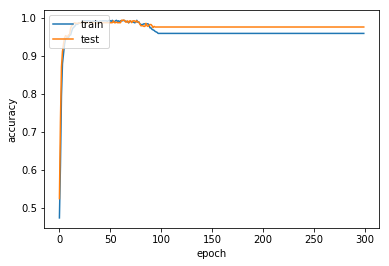
\includegraphics[width=80mm]{banknote_forgery_files/hidden1}
\end{minipage}\hfill
\begin{minipage}[b]{0.5\linewidth}
\centering
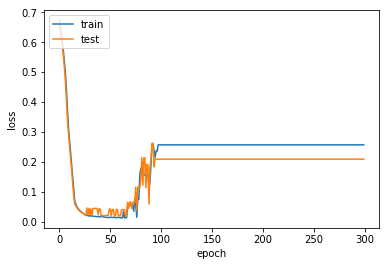
\includegraphics[width=80mm]{banknote_forgery_files/hidden2}
\end{minipage}
\end{table}





\subsubsection{Implementing Dropout} Since the analysis summarized in \S 2. \ref{conc1} showed that the data is prone to overfitting, as a final step we investigate if adding a Dropout layer improves our model. This drastic technique is typically used to prevent overfitting in deep nets trained on large datasets and consists of deactivating neurons at random (according to a probability rate) in order to force the model to keep learning. This functionality can be implemented easily in \texttt{keras} through the command \texttt{model.add(Dropout())}.  For the benefit of the reader, we include the psuedocode for our final algorithm:
\begin{algorithm}
    \SetKwInOut{Output}{Output}
	model$()$\;
    \Output{a fitted neural net with an Adam optimizer, hidden layer and Dropout}
    model=Sequential$()$\\
	model.add(Dense(4,input\un dim=4,activation='sigmoid'))\\
	model.add(Dropout(0.5))\\
	model.add(Dense(2,input\un dim=4,activation='sigmoid'))
	history=comp\un fit(logmodel,'Adam',300)\\
	learning\un curves(history)\\
   \caption{logistic regression in \texttt{keras} }
\end{algorithm}


After adding a Dropout layer between the input and hidden layer, the learning curves were as follows:
\begin{table}[ht]
\begin{minipage}[b]{0.3\linewidth}
\centering
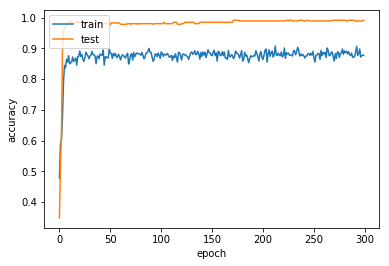
\includegraphics[width=80mm]{banknote_forgery_files/dropout_1}
\end{minipage}\hfill
\begin{minipage}[b]{0.5\linewidth}
\centering
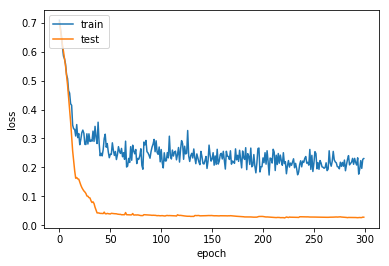
\includegraphics[width=80mm]{banknote_forgery_files/dropout_2}
\end{minipage}
\end{table}

\noindent The learning curves for the training set are more stochastic in  nature, due to the randomness inherent to the Dropout method. We can see that the method did produce favorable results as the accuracy on the testing set is 99\%

\section{Summary}

We began our investigation of the problem by preprocessing the data through the use of various statistical- and machine learning techniques which allowed us to gain insight into the data's nature.\\ Along the way, we descovered that the features were equidistributed,; we detected and removed the necessary outliers; showed that precisely two features were significantly correlated; reduced the dimension to gain visual insight and determined that a simply clustering technique would not be be suitable for this problem.\\\\ 
In the second stage of our research, we built a neural net to classify the data using \texttt{keras}. After implementing a first approximate model based off logistic regression, the learning curves showed that adapting the optimizer would yield better results. After lowering the learning rate, we obtained a model that indeed showed a lower cost, but did not improve on accuracy. We then added a second hidden layer with 4 input nodes to the net, based off trial and error. Finally, based on the idea that the data could be overfitted, we added a dropout layer, which resulted in a model that has a 99\% accuracy:

\begin{center}
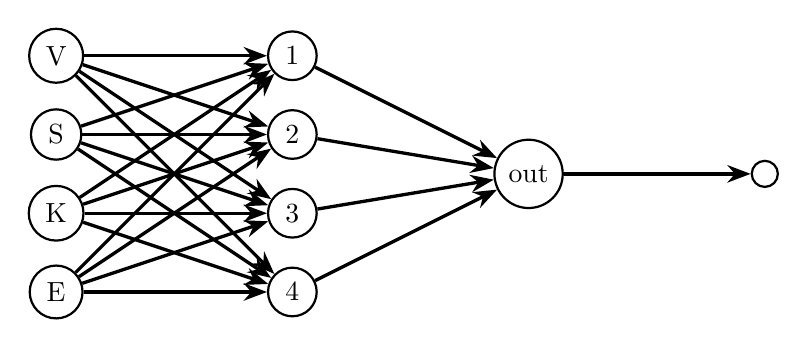
\begin{tikzpicture}
\begin{scope}[every node/.style={circle,thick,draw}]
    \node (A) at (0,0) {V};
    \node (B) at (0,-1) {S};
    \node (C) at (0,-2) {K};
    \node (D) at (0,-3) {E};
    \node (E) at (3,0) {1};
    \node (J) at (3,-1) {2};
    \node (F) at (3,-2) {3};
    \node (G) at (3,-3) {4};
    \node (H) at (6,-1.5) {out};
    \node (I) at (9,-1.5) {};
\end{scope}

\begin{scope}[>={Stealth[black]},
              every node/.style={fill=white,circle},
              every edge/.style={draw=black,very thick}]
    \path [->] (A) edge (E);
    \path [->] (A) edge (J);
    \path [->] (A) edge (F);
    \path [->] (A) edge (G);
    \path [->] (B) edge (E);
    \path [->] (B) edge (J);
    \path [->] (B) edge (F);
    \path [->] (B) edge (G); 
    \path [->] (C) edge (E);
    \path [->] (C) edge (J);
    \path [->] (C) edge (F);
    \path [->] (C) edge (G);
    \path [->] (D) edge (E);
    \path [->] (D) edge (J);
    \path [->] (D) edge (F);
    \path [->] (D) edge (G);
    \path [->] (E) edge (H);
    \path [->] (J) edge (H);
    \path [->] (F) edge (H);
    \path [->] (G) edge (H);  
    \path [->] (H) edge (I); 
    \end{scope}
\end{tikzpicture}
\end{center}

\noindent In conclusion, given a scanned banknote, we believe that this model is capable of accurately detecting foul play given the statistical features of an image.
 

\addcontentsline{toc}{section}{References}

\bibliographystyle{alpha}
\bibliography{banknote_forgery_bib}
\end{document}
